
\documentclass[12pt]{article}
\usepackage[T1]{fontenc}
% \usepackage{babel}
\usepackage{titling}
\usepackage{blindtext}
\usepackage{geometry}
\usepackage{hyperref}
\usepackage{float}

\usepackage{epsfig}
\usepackage{graphicx}


\setlength{\droptitle}{-6em}     % Eliminate the default vertical space
\addtolength{\droptitle}{-4pt}   % Only a guess. Use this for adjustment

\title{\Large \bf 2.152 Project: \\ Adaptive Control of 2-Link Robotic Arm}
\author{\vspace{-6em}Luke Roberto}
\date{\vspace{-4em}May 14th, 2018}
\maketitle

\begin{document}

\vspace{-2em}

%%%%%%%%%%%%%%%%%%%%%%%%%%%%%%%%%%%%%%%%%%%%%%%%%%%%%%%%%%%%%%%%%%%%%%%%%%%%%%%%%%%%%%%%
\section{Setup}

The purpose of this project was to implement composite adaptive control on an interesting system while also learning to use the Julia programming language. The project code is located at: \url{https://github.com/Lukeroberto/2.152_project}. There are a collection of Julia Notebooks that can be viewed without actually installing the language on your system, you can also view short gifs of the results as well. I made use of the Julia Robotics toolkit, a very helpful package which provides an abundance of functionality from visualization to automatic equations of motion generation from description files.

%%%%%%%%%%%%%%%%%%%%%%%%%%%%%%%%%%%%%%%%%%%%%%%%%%%%%%%%%%%%%%%%%%%%%%%%%%%%%%%%%%%%%%%%
\section{Adaptive Control of Double Integrator}

The first steps of this project were to model a simple system. This allowed me a little time to get comfortable with the language and build intuition on how the adaptive controller worked realtime. The double integrator plant and controller that I used is as follows:
$$
Model: m\ddot{x} = \tau
$$
$$
Control Law: \tau = \hat{m}(\ddot{x_d} - 2\lambda \dot{\tilde{x}} - \lambda^2  \tilde{x})
$$
$$
Adaptation Law: \dot{\hat{m}} = -\gamma v s
$$
\\

\begin{figure}[H]
    \centering
    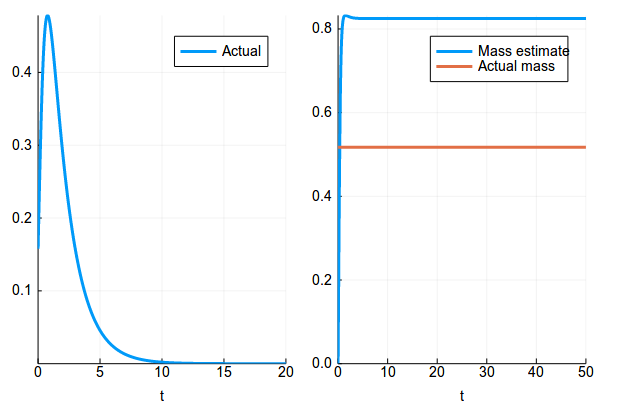
\includegraphics[width=3.5in\textsize]{sufficient_richness.png}
    \caption{Set point control}
    \label{fig:double_integrator_suff}
\end{figure}

\newpage
\noindent
I then used this scheme to do trajectory tracking of the double integrator. The first test was to simply send the system to the origin. This proved to be an interesting test of sufficient richness. Fig. 1 shows we have nice exponential convergence to the origin, but do not converge on the correct value of the mass. The trajectory is not sufficiently rich because it only requires the controller to push the system in one direction, it is not until we have  a more interesting error signal to extract information from that we can converge on the true value of the mass.
\\

\begin{figure}[H]
    \centering
    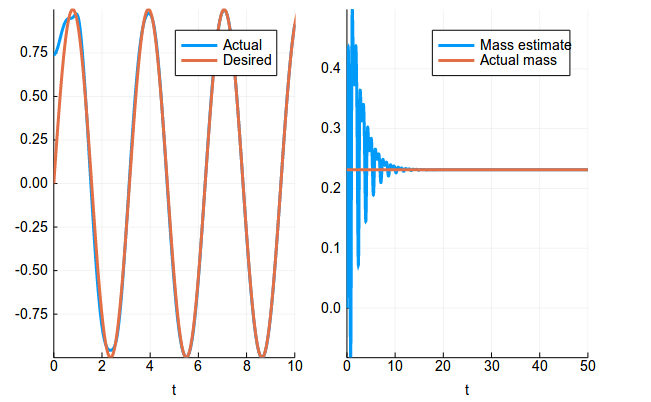
\includegraphics[width=3.5in\textsize]{double_integrator_adaptation.png}
    \caption{Tracking $sin(2t)$}
    \label{fig:double_integrator_sine}
\end{figure}

\noindent
Fig. 2 shows the controller tracking $sin(2t)$. There is nice exponential convergence as expected, although intuitively it is interesting to me how the controller has essentially zero error around $t=4$, yet does not learn the mass until approximately $t=15$. I assume the nature of the controller has a good deal of robustness, especially when the mass estimate error shrinks below a sufficient threshold.
\\

\begin{figure}[h]
    \centering
    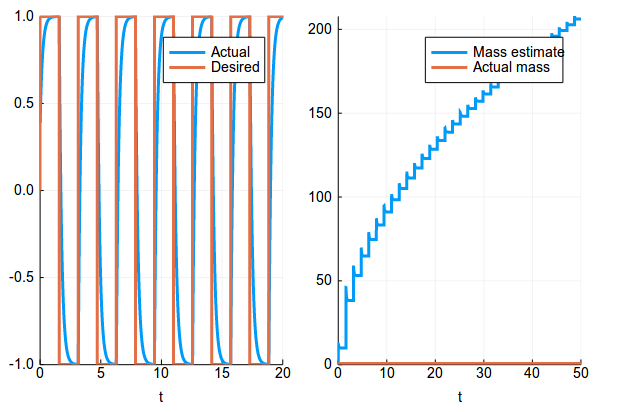
\includegraphics[width=3.5in\textsize]{double_integrator_square_wave.png}
    \caption{Tracking $sgn(sin(2t))$}
    \label{fig:double_integrator_sq}
\end{figure}

\noindent
After testing out the controller on a trivial set of trajectories, I decided to see what would happen if I were to break some of the assumptions that were made in the derivations of adaptive control. The most interesting one in my opinion is shown in Fig. 3. The desired trajectory is a square wave of the same frequency as the previous input. The closed loop system behaves like a second order system trying to follow a square wave input, even though the mass estimate grows unbounded. This may be an artifact of the implementation, but an interesting observation nonetheless.
\\


%%%%%%%%%%%%%%%%%%%%%%%%%%%%%%%%%%%%%%%%%%%%%%%%%%%%%%%%%%%%%%%%%%%%%%%%%%%%%%%%%%%%%%%%
\section{Adaptive Control of 2-Link Arm}

Once I was able to test out the double integrator system, I then moved on to control of the 2-link arm dynamics as specified in example 9.1 of the textbook. For the sake of having a ground truth to compare my results against initially, I used the same masses, inertias, and lengths as the example problems. This proved useful in debugging, and made the lengthy process of developing this model a little easier.
\\


\begin{figure}[H]
    \centering
    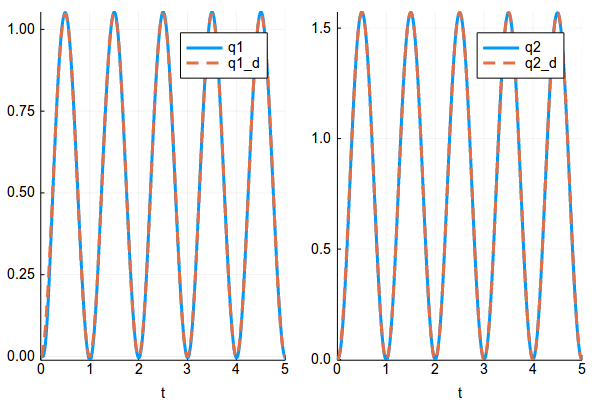
\includegraphics[width=3.5in\textsize]{arm_trajectory_tracking2.png}
    \caption{Trajectory tracking}
    \label{fig:arm1}
\end{figure}

\noindent
Fig. 4 shows the successful trajectory tracking controller implemented on the system. The convergence rate is as expected for the large $ K_d$ and $\lambda$ values specified, and tracks very well for the duration of the simulation.

\begin{figure}[H]
    \centering
    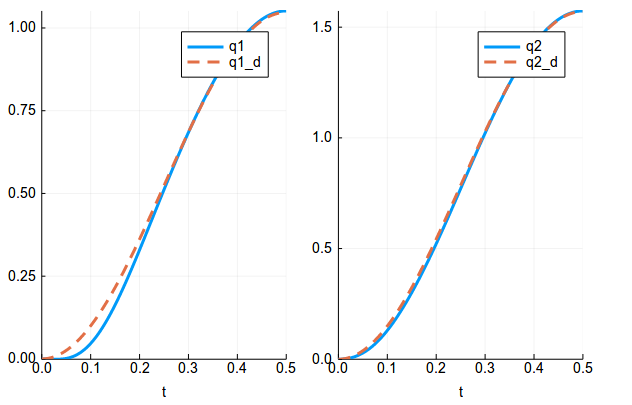
\includegraphics[width=3.5in\textsize]{arm_trajectory_tracking.png}
    \caption{Trajectory tracking (smaller timescale)}
    \label{fig:arm2}
\end{figure}

\noindent
Upon closer inspection, as seen in Fig. 5, the convergence happens in approximately two tenths of a second.
\\

\noindent
I then turned my attention to the parameter estimates. One thing I had not thought of before seeing the equations of motion was the fact that there are only 4 linear parameters to which we can adapt. This means I could actually not back out the mass of the object with adaptation as I had originally planned to do. The best we can do is learn $a_2$, which is the effective inertial contribution from the second link and object combined.

\begin{figure}[H]
    \centering
    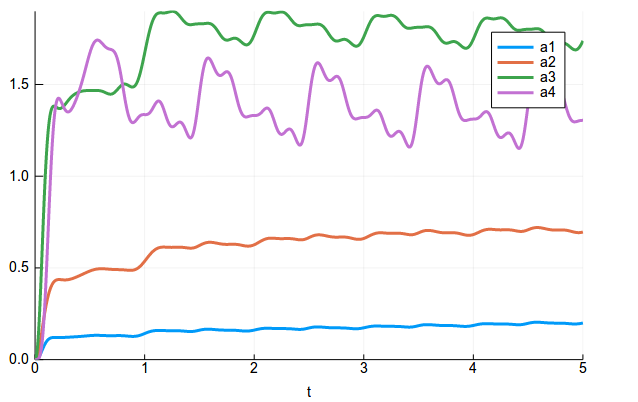
\includegraphics[width=3.5in\textsize]{arm_parameter_estimates.png}
    \caption{Estimated arm parameters}
    \label{fig:arm_param}
\end{figure}

\noindent
The other thing that I noticed is demonstrated in Fig. 6. The paramater estimates stabilize at rather large periodic trajectories, and also do not seem to be estimating the correct values of the parameter vector. This makes some sense though, because the only thing that matters to the actual control of the object is the product Ya. I also noticed that the controller was somewhat sensitive to trajectories that I commanded, some of them would not track as well as others.
\\
%%%%%%%%%%%%%%%%%%%%%%%%%%%%%%%%%%%%%%%%%%%%%%%%%%%%%%%%%%%%%%%%%%%%%%%%%%%%%%%%%%%%%%%%
\section{Composite Adaptive Control}

Unfortunately, I did not have the time to fully implement composite adaptive control with bounded gain forgetting on the manipulator model. There is code in place that could perform the parameter estimation, but there are a few issues I was unable to track down. It was interesting to see how big the state space model got when I added the composite controller, 8 states in the simple adaptive case to approximately 20 states in the composite case. It took a long time for my computer to integrate these trajectories, and so debugging became a time issue. I did spend a good portion of my time reading the last portions of chapter 8 and chapter 9 to understand the derivations of the different types of parameter estimation. It would definitely be beneficial for me to go back at some point and try to get this working on the current model. Smoothing out the fluctuations in the estimated parameters and also testing robustness to slowly-varying parameters would be interesting directions to continue this project.
\\
%%%%%%%%%%%%%%%%%%%%%%%%%%%%%%%%%%%%%%%%%%%%%%%%%%%%%%%%%%%%%%%%%%%%%%%%%%%%%%%%
\section{Concluding Remarks}

In conclusion, I have really enjoyed the work that I have done for this project so far. Adaptive control seems to be a very rich field that I have only scratched the surface. I was able to implement simple algorithms that gave me really powerful results.
\\

\noindent
One thing I definitely want to look into for the future is if there has been research into making adaptive control less computationally intensive online. For the simple 2-link robotic arm in the example, the state space when from 4DOF to 8DOF once adaptive control was added. My attempt at implementing composite adaptive control with bounded-gain forgetting had a state space model that had more than 16 state variables to keep track of all the dynamics. I believe that this would be difficult to implement on a system that was sufficiently more complex than this one.
\\

\noindent
My favorite aspect of adaptive control is the verifcation that you get with the lyapunov function. You can provably prove convergence of these systems even when the parameters are unknown. If you use basis function expansions, you could even have entire models be unknown. This is very powerful to me. I will be starting graduate work in the fall in robotic manipulation. I feel like much of this field has moved in the direction of model-free approaches like Reinforcement learning, so it would be nice to see if we develop algorithms more like adaptive control that are not so data hungry and have some sort of guarantee of stability/convergence. Thank you very much for a wonderfully taught class, I will definitely be referencing this material often!
\\

\end{document}
